%
% Elliott Hudson College - Maths Booklet Template
% Originally created on: May 3rd 2021
%
% Copyright (C) 2021 Ellis Dickinson
%
% LICENSE:
% This program is free software: you can redistribute it and/or modify
% it under the terms of the GNU General Public License as published by
% the Free Software Foundation, either version 3 of the License, or
% any later version.
%
% This program is distributed in the hope that it will be useful,
% but WITHOUT ANY WARRANTY; without even the implied warranty of
% MERCHANTABILITY or FITNESS FOR A PARTICULAR PURPOSE.  See the
% GNU General Public License for more details.
%
% You should have received a copy of the GNU General Public License
% along with this program. If not, see <https://www.gnu.org/licenses/>.
%
%
% IMPORTANT!!!!
% When compiling this document, please use XeLaTeX
% Other compilers do not support some of the features within this document.
%
\documentclass[fleqn]{article}

\usepackage{relsize}
\usepackage{tabulary}

\setcounter{section}{6}                                          % Set the Unit Number (without Leading 0's)
\newcommand{\coursetitle}{A-Level Further Mathematics}           % Set the Course Title
\newcommand{\bookletunittitle}{Chi-Squared Tests}                % Set the Unit Title
\newcommand{\bookletsubtitle}{Content last revised by: S Waugh}  % Set the Subtitle
\newcommand{\unitprefix}{FS}                                     % Set the Unit Prefix

% DO NOT MODIFY THIS FIILE
% ----------------------------------------------
\usepackage[dvipsnames]{xcolor}
\usepackage[a4paper, portrait, margin=1.9cm]{geometry}
\usepackage{titlesec}
\usepackage{tikz}\usetikzlibrary{shapes.misc}\usetikzlibrary{calc}
\usepackage{setspace}
\usepackage{fontspec}
\usepackage[most]{tcolorbox}
\usepackage{varwidth}
\usepackage[inline]{enumitem}
\usepackage{multicol}
\usepackage{fancyhdr}
\usepackage{booktabs, tabularx}
\usepackage{mathtools}
\usepackage{tasks}
\usepackage{anyfontsize}
\usepackage[export]{adjustbox}		% http://ctan.org/pkg/adjustbox




\newcounter{taskscounter}
\settasks{							% Multi-column enumeration
	style=enumerate,
	counter=taskscounter,
	label-width={22pt},
	item-indent={15pt},
	label-align=right,
	label=\textbf{\alph*},
	before-skip = -\parskip , 		% undo paragraph skip
  	after-skip = -\parskip , 		% undo paragraph skip
  	after-item-skip = -\parskip+1mm	% undo paragraph skip
%   debug=true 						% useful for fine-tuning or debugging
}



% Define dynamic titlebars for sections/exercises
\newlength{\sectionnumberwidth}
\newcommand\titlebar{\hspace*{-0.1cm}
	\tikz[baseline, trim right=3.1cm] {
		\settowidth{\sectionnumberwidth}{
			\pgfinterruptpicture
				\textbf{\sffamily\thesection.\thesubsection}
			\endpgfinterruptpicture
		}
	    \fill [cyan!25, rounded corners=0.15cm] (2.5cm,-1.28ex) rectangle (\textwidth-\sectionnumberwidth+2.65cm,2.615ex);
	    \node [
	        fill=blue!60!white,
	        text=white,
	        anchor= base east,
	        rounded rectangle,
	        inner sep = 2mm,
	        minimum height=3.89ex] at (3cm,0) {
	        {\bfseries\thesection.\thesubsection}
	    };
	}
}
\newcommand\exercisebar{\hspace*{-0.1cm}
	\tikz[baseline, trim right=3.1cm] {
		\settowidth{\sectionnumberwidth}{
			\pgfinterruptpicture
				\textbf{\sffamily\thesection.\thesubsubsection}
			\endpgfinterruptpicture
		}
	    \fill [red!25, rounded corners=0.15cm] (2.5cm,-1.265ex) rectangle (\textwidth-\sectionnumberwidth+2.65cm,2.64ex);
	    \node [
	        fill=cherryred!80!white,
	        text=white,
	        anchor= base east,
	        rounded rectangle,
	        inner sep = 2mm,
	        minimum height=3.9ex] at (3cm,0) {
	        {\bfseries\thesection\thesubsubsection}
	    };
	}
}

\newtcolorbox{mybox2}[2][]{
	enhanced,
	before skip=2mm,after skip=2mm,
	colback=black!5,
	colframe=black!50,
	boxrule=0.2mm,
	attach boxed title to top left={
		xshift=1cm,yshift*=1mm-\tcboxedtitleheight},
		varwidth boxed title*=-3cm,
		boxed title style={frame code={
            \path[fill=tcbcolback!30!black]
              ([yshift=-1mm,xshift=-1mm]frame.north west)
                arc[start angle=0,end angle=180,radius=1mm]
              ([yshift=-1mm,xshift=1mm]frame.north east)
                arc[start angle=180,end angle=0,radius=1mm];
            \path[left color=tcbcolback!60!black,right color=tcbcolback!60!black,
              middle color=tcbcolback!80!black]
              ([xshift=-2mm]frame.north west) -- ([xshift=2mm]frame.north east)
              [rounded corners=1mm]-- ([xshift=1mm,yshift=-1mm]frame.north east)
              -- (frame.south east) -- (frame.south west)
              -- ([xshift=-1mm,yshift=-1mm]frame.north west)
              [sharp corners]-- cycle;
            },interior engine=empty,
          },
	fonttitle=\sffamily\bfseries,
    title={#2},
    before upper = \sffamily,
    #1
}
          
\tcbset{%
    example/.style={%
        enhanced,
        breakable,
        rounded corners,
        toprule=0pt, rightrule=0pt, bottomrule=0pt, leftrule=1mm,
        colback=#1!5, colframe=#1!80!black, coltitle=#1!80!black,
        fonttitle=\bfseries\large\sffamily,
        detach title,
        before upper={\tcbtitle\quad},
        fontupper=\linespread{1.2}\selectfont
    },
    note/.style={%
        enhanced,
        breakable,
        separator sign none,
        rounded corners,
        toprule=0pt, rightrule=0pt, bottomrule=0pt, leftrule=1mm,
        colback=#1!5, colframe=#1!80!black, coltitle=#1!80!black,
        fonttitle=\bfseries\large,
        detach title,
        before upper={\sffamily\tcbtitle\quad\hspace{-2mm}},
        fontupper=\linespread{1.2}\selectfont
    }
}
\newtcbtheorem[auto counter]{examplebox}{Example}
{example=blue}{ex}
\newtcbtheorem{practice}{Independent Practice}
{example=practiceorange}{pr}
\newtcbtheorem{note}{#1\hspace{-1mm}}
{note=notecolor}{nt}



% Custom Colour Definitions
\definecolor{practiceorange}{RGB}{252, 191, 0}
\definecolor{notecolor}{RGB}{0, 0, 0}
\definecolor{cherryred}{RGB}{191,0,0}

\definecolor{ehclogoblue}{RGB}{0,187,211}
\definecolor{ehclogogray}{RGB}{33, 34, 33}
\definecolor{ehclogoorange}{RGB}{243, 108, 33}
\definecolor{separatorgray}{RGB}{210, 210, 210}



\setstretch{1.1} 										% Globally adjust bullet spacing
\setlength{\parindent}{0cm} 								% Removes paragraph indent
\setlength{\multicolsep}{6.0pt plus 2.0pt minus 1.5pt}	% Halves whitespace before multicol environment
\setlength\tabcolsep{0pt} 								% Removes default space between columns in table

% Change various spacings of bulleted/numbered lists
\setlist[itemize]{topsep=2pt, itemsep=-2pt}
\setlist[enumerate]{topsep=-2pt, partopsep=4mm, itemsep=0pt}

% Change spacing of aligned mathematics
\AtBeginDocument{
	\setlength\abovedisplayskip{3pt}
	%\setlength{\belowdisplayskip}{0pt}
	\setlength\belowdisplayskip{7pt}
	%\setlength{\belowdisplayshortskip}{0pt}
}


\setsansfont{AptiferSansPro}[
	Path = fonts/,
	Extension = .ttf,
    UprightFont = *-Regular,
    BoldFont = *-Medium
]



% Implement the custom titlebars
\titleformat{\section}{\large\sffamily}{\titlebar}{0.1cm}{}
\titleformat{\subsection}{\large\sffamily}{\titlebar}{0.1cm}{}
\titleformat{\subsubsection}{\large\sffamily}{\exercisebar}{0.1cm}{}



% Define the easier get functions for sections and subsections
\renewcommand*{\thesection}{\arabic{section}}
\renewcommand*{\thesubsection}{\arabic{subsection}}
\renewcommand*{\thesubsubsection}{\Alph{subsubsection}}
\newcommand\getcurrentref[1]{%
 \ifnumequal{\value{#1}}{0}
  {??}
  {\the\value{#1}}%
}
\newcommand{\exercise}{\subsubsection}



%Custom font size 'YUGE', larger than huge
\newcommand\YUGE{\fontsize{35}{35}\selectfont}

% Define custom footer
\fancypagestyle{plain}{
	\fancyhf{} % clear all header and footer fields
	\fancyfoot[OC]{ %right hand side
		\vspace{-0.7em}
		\hfill {\sffamily\raggedright {\color{separatorgray}\getcurrentref{page}} \\}\vspace{-1.6em}
		\begin{minipage}{.3\linewidth}
			\color{separatorgray}\rule{\linewidth}{0.4pt}
		\end{minipage}
		\begin{minipage}{.1\linewidth}
			\centering
			
\includegraphics[scale=0.4]{images/ehc-brand-separator-icon}
		\end{minipage}
		\begin{minipage}{.3\linewidth}
			\color{separatorgray}\rule{\linewidth}{0.4pt}
		\end{minipage}
	}
	\fancyfoot[EC]{ %left hand side
		\vspace{-0.7em}
		{\sffamily\raggedright {\color{separatorgray}\getcurrentref{page}} \\}\vspace{-1.6em}
		\begin{minipage}{.3\linewidth}
			\color{separatorgray}\rule{\linewidth}{0.4pt}
		\end{minipage}
		\begin{minipage}{.1\linewidth}
			\centering
			
\includegraphics[scale=0.4]{images/ehc-brand-separator-icon}
		\end{minipage}
		\begin{minipage}{.3\linewidth}
			\color{separatorgray}\rule{\linewidth}{0.4pt}
		\end{minipage}
	}

	\renewcommand{\headrulewidth}{0pt}
	\renewcommand{\footrulewidth}{0pt}
}
\pagestyle{plain}



% Function for adding vspace above underbrace
\newcommand*\addunderbracespace[1]{\vrule width0pt height0pt depth#1\relax}


\newcommand{\formattedunittitle}{Unit P\getcurrentref{section}}

\bluetheme

% Preamble Overrides
\setlength{\tabcolsep}{1mm}

% Document Content Starts Here
\begin{document}
% DO NOT MODIFY THIS FIILE
% ----------------------------------------------
% Title Page
% ----------------------------------------------
% Modified from a post from a post by ModyTex
% https://www.reddit.com/r/LaTeX/comments/faij1n/my_first_cover_page_done_in_latex_is_it/
% ----------------------------------------------
\pagestyle{empty}
\begin{tikzpicture}[overlay,remember picture]
    \begin{scope}[transform canvas ={rotate around ={45:($(current page.north)+(-1.5,-3)$)}}]
    \shade[rounded corners=12pt, left color=gray!80, right color=gray!80] ($(current page.north)+(-2,-6.7)$) rectangle ++(9,0.8);
    \end{scope}

    \begin{scope}[transform canvas ={rotate around ={45:($(current page.north)+(-3,-8)$)}}]
    \shade[rounded corners=20pt, left color=lightgray!80, right color=lightgray!80] ($(current page.north)+(2.5,-8)$) rectangle ++(15,1.35);
    \end{scope}

    \begin{scope}[transform canvas ={rotate around ={45:($(current page.north west)+(4,-15.5)$)}}]
    \shade[rounded corners=20pt, left color=ehclogoorange, right color=ehclogoorange] ($(current page.north west)+(15,-16)$) rectangle ++(20,1.5);
    \end{scope}

    \begin{scope}[transform canvas ={rotate around ={45:($(current page.north west)+(13,-10)$)}},]
    \shade[rounded corners=18pt, left color=ehclogoblue ,right color=ehclogoblue] ($(current page.north west)+(14.5,-10)$) rectangle ++(15,1.3);
    \end{scope}

    \begin{scope}[transform canvas ={rotate around ={45:($(current page.north west)+(18,-8)$)}},]
    \shade[rounded corners=8pt, left color=ehclogogray, right color=ehclogogray] ($(current page.north west)+(18.5,-8)$) rectangle ++(15,0.6);
    \end{scope}

    \begin{scope}[transform canvas ={rotate around ={45:($(current page.north west)+(19,-5.65)$)}},]
    \shade[rounded corners=12pt, left color=lightgray, right color=lightgray] ($(current page.north west)+(15.5,-5.65)$) rectangle ++(15,0.8);
    \end{scope}

    \begin{scope}[transform canvas ={rotate around ={45:($(current page.north west)+(20,-9)$)}}]
    \shade[rounded corners=15pt, left color=ehclogoorange, right color=ehclogoorange] ($(current page.north west)+(20,-8.4)$) rectangle ++(14,1.1);
    \end{scope}
\end{tikzpicture}

\vspace{-0.5cm}

\includegraphics{images/branding/brand-logo-vector}

\vspace{8.5cm}
\begin{minipage}{\textwidth}
    \sffamily

    \vspace{2mm}
    {\YUGE \raggedleft\bookletunittitle\\}

    \vspace{1mm}
    {\huge \raggedleft\coursetitle { }-- \formattedunittitle\\}

    \vspace{2mm}
    {\small \raggedleft\bookletsubtitle\\}
\end{minipage}
\vfill
% Key Information
% ----------------------------------------------

\begin{adjustbox}{valign=b}
	\begin{minipage}{.85\textwidth}
		\begin{mybox2}[colbacktitle=green]{Key Information}
			\textbf{Key Formulae:}
			\[
			\begin{aligned}
				x^a \times x^b &= x^{a+b} \\
				x^a \div x^b &= x^{a-b} \\
				(x^a)^b &= x^{ab} \\
				x^{-n} &= \dfrac{1}{x^n} \\
				x^{\tfrac{1}{n}} &= \sqrt[\textstyle{^n}]{x} \\
				a^2 - b^2 &= (a-b)(a+b)
			\end{aligned}
			\]

			\textbf{Key Terms:}
			\begin{itemize}
				\item \textbf{Expanding Brackets:} Multiplying brackets out
				\item \textbf{Factorising Brackets:} Putting expressions back into brackets
				\item \textbf{Surd:} A root of a number which can't be written as a whole number or fraction
				\item \textbf{Rationalising Denominator:} Removing the surd from the bottom of the fraction
			\end{itemize}
		\end{mybox2}
	\end{minipage}
\end{adjustbox}
\begin{minipage}[b]{.13\textwidth}
	\sffamily
	Solution Bank:
	\vspace{1mm}\linebreak
	
\includegraphics[scale=0.15, valign=b]{images/link-to-y1-sol-bank}
\end{minipage}


\begin{keyinformation}{images/link-to-y1-sol-bank}
    \begin{enumerate}
        \item The \textbf{null} and \textbf{alternative hypotheses} generally take the following form:        \\
            H\textsubscript{0}: There is no difference between the observed and the theoretical distribution. \\
            H\textsubscript{1}: There is a difference between the observed and the theoretical distribution.
        \item \textbf{Goodness of fit} is concerned with measuring how well and observed frequency distribution fits to a known distribution.
        \item The measure of \textbf{goodness of fit} is $X^2={\mathlarger{\sum}} \dfrac{(O_i-E_i)^2}{E_i}$ or $X^2={\mathlarger{\sum}} \dfrac{O_i^2}{E_i}-N$
        \item The $\chi^2$ family of distributions can b used to approximate $X^2$ as long as none of the expected values is below 5.
        \item When calculating \textbf{degrees of freedom:} \vspace{2mm}\\
            $v$ = number of cells after combining $-$ number of constraints \vspace{1mm}
        \item When using chi-squared tests, if any of the expected values are less than 5, then you have to combine frequencies in the data table until they are greater than 5.
        \item When selecting which of the $\chi^2$ family to use as an approximation for $X^2$, you have to select the distribution which has $v$ equal to the number of degrees of freedom of your expected values.
        \item If $X^2$ exceeds the critical value, it is unlikely that the null hypothesis is correct so you reject it in favour of the alternative hypothesis.
    \end{enumerate}
\end{keyinformation}

\newpage
\pagestyle{attribution}


% TODO Links to the Big Picture
\begin{mybox2}[colbacktitle=WildStrawberry]{Links to the Big Picture}
    \begin{enumerate}[label*=\bfseries \unitprefix\arabic*., leftmargin=*]
        \setcounter{enumi}{\getcurrentref{section}-1}
        \item \textbf{\bookletunittitle}
        \begin{enumerate}[label*=\bfseries\arabic*]
            % Unit Components Go Here
            \item Goodness of Fit
            \item Testing a Hypothesis
            \item Testing with Discrete Distributions (Parameter Known)
            \item Testing with Discrete Distributions (Parameter Unknown)
            \item Using Contingency Tables
        \end{enumerate}
    \end{enumerate}
    Develops:
    \begin{itemize}
        \item Hypothesis Testing
        \item Estimating Parameters (Expectation and Variance)
    \end{itemize}
    \vspace{1mm}
\end{mybox2}

\newpage
\pagestyle{branded}



\lesson{Goodness of Fit}


\begin{mybox2}[colbacktitle=WildStrawberry]{Summary}
    \setlength{\parskip}{0.5\baselineskip}%
    \textbf{Goodness of fit} is concerned with measuring how well an observed frequency distribution fits to a known distribution.
    
    Suppose you take a dice and throw it 120 times. You might get results like these:
    \begin{center}\vspace{-2mm}
    \begin{minipage}[t]{0.8\linewidth}
        \begin{tabularx}{\textwidth}{|X|>{\centering\arraybackslash}p{11mm}|>{\centering\arraybackslash}p{11mm}|>{\centering\arraybackslash}p{11mm}|>{\centering\arraybackslash}p{11mm}|>{\centering\arraybackslash}p{11mm}|>{\centering\arraybackslash}p{11mm}|}
            \hline
            \textbf{Number on dice, n} & 1 & 2 & 3 & 4 & 5 & 6                      \\\hline
            \textbf{Observed frequency ($O_i$)} & 23 & 15 & 25 & 18 & 21 & 18       \\\hline
        \end{tabularx}
    \end{minipage}
    \end{center}
    
    If the dice is \textit{unbiased} you would, in theory, expect each of the numbers 1 to 6 to appear the same number of times.
    
    For 120 throws the expected frequencies would each be:
    
    \hspace{1cm} $P(X=x) \times 120 = \dfrac{1}{6} \times 120 = 20$
    
    You would expect results like these:
    
    \begin{center}\vspace{-2mm}
    \begin{minipage}[t]{0.8\linewidth}
        \begin{tabularx}{\textwidth}{|X|>{\centering\arraybackslash}p{11mm}|>{\centering\arraybackslash}p{11mm}|>{\centering\arraybackslash}p{11mm}|>{\centering\arraybackslash}p{11mm}|>{\centering\arraybackslash}p{11mm}|>{\centering\arraybackslash}p{11mm}|}
            \hline
            \textbf{Number on dice, n} & 1 & 2 & 3 & 4 & 5 & 6                      \\\hline
            \textbf{Observed frequency ($O_i$)} & 20 & 20 & 20 & 20 & 20 & 20       \\\hline
        \end{tabularx}
        \vspace{4mm}
    \end{minipage}
    \end{center}
    
    \begin{itemize}
        \bfseries
        \item H\textsubscript{0}: There is no difference between the observed and the theoretical distribution.
        \item H\textsubscript{1}: There is a difference between the observed and the theoretical distribution.
    \end{itemize}
    
    In order to tell how closely the model fits the observed results you need to have a measure of the \\\textbf{goodness of fit} between the observed frequencies and the expected frequencies.
    
    The results and the expected frequencies are:
    
    \begin{center}\vspace{-2mm}
    \begin{minipage}[t]{0.8\linewidth}
        \begin{tabularx}{\textwidth}{|X|>{\centering\arraybackslash}p{11mm}|>{\centering\arraybackslash}p{11mm}|>{\centering\arraybackslash}p{11mm}|>{\centering\arraybackslash}p{11mm}|>{\centering\arraybackslash}p{11mm}|>{\centering\arraybackslash}p{11mm}|}
            \hline
            \textbf{Number on dice, n} & 1 & 2 & 3 & 4 & 5 & 6                      \\\hline
            \textbf{Observed frequency ($O_i$)} & 23 & 15 & 25 & 18 & 21 & 18       \\\hline
            \textbf{Observed frequency ($O_i$)} & 20 & 20 & 20 & 20 & 20 & 20       \\\hline
        \end{tabularx}
        \vspace{4mm}
    \end{minipage}
    \end{center}
    
    
    \textbf{The measure of goodness of fit is:}
    
    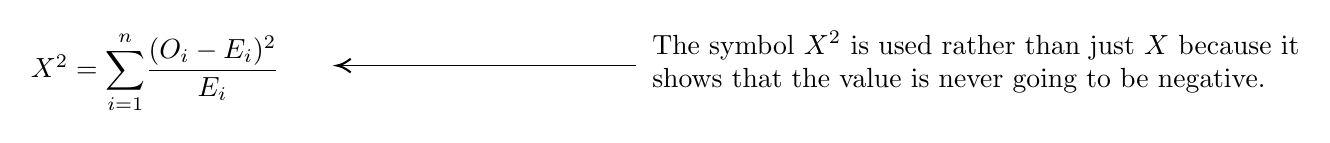
\begin{tikzpicture}[x=0.75pt,y=0.75pt,yscale=-1,xscale=0.6]
        % Shape: Boxed Line [id:dp5924871900366302] 
        \draw (490,21) -- (250,21) ;
        \draw [shift={(250,21)}, rotate = 360.07] [color=black][line width=0.75]    (10.93,-3.29) .. controls (6.95,-1.4) and (3.31,-0.3) .. (0,0) .. controls (3.31,0.3) and (6.95,1.4) .. (10.93,3.29)   ;
        
        % Text Node
        \draw (2,3.4) node [anchor=north west][inner sep=0.75pt]{%
            $X^{2} ={\mathlarger\sum _{i=1}^{n}}\dfrac{( O_{i} -E_{i})^{2}}{E_{i}}$
        };
        
        % Text Node
        \draw (501,3) node [anchor=north west][inner sep=0.75pt][align=left]{%
            The symbol $\displaystyle X^{2}$ is used rather than just $\displaystyle X$ because it\\
            shows that the value is never going to be negative.};
    \end{tikzpicture}
    
    You can see that the less good the fit, the larger the difference between each observed and expected value, and the greater the value of $X^2$.
    
    
    \textbf{Here is another way of calculating $X^2$:}
    
    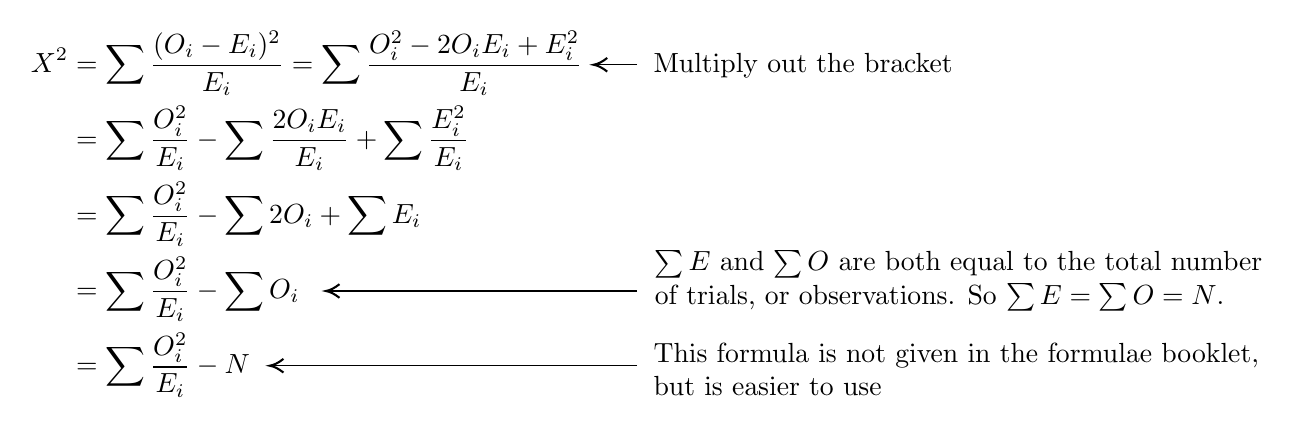
\begin{tikzpicture}[x=0.75pt,y=0.75pt,yscale=-1,xscale=0.6]
        % Uncomment if require:
        % \path (0,354);  % Set diagram left start at 0, and has height of 354
        
        % Straight Lines [id:da18451996657129888] 
        \draw (490,102) -- (455,102) ;
        \draw [shift={(455,102)}, rotate = 360] [color=black][line width=0.75]    (10.93,-3.29) .. controls (6.95,-1.4) and (3.31,-0.3) .. (0,0) .. controls (3.31,0.3) and (6.95,1.4) .. (10.93,3.29)   ;
        % Straight Lines [id:da645763229182968] 
        \draw (490,211) -- (240,211) ;
        \draw [shift={(240,211)}, rotate = 360] [color=black][line width=0.75]    (10.93,-3.29) .. controls (6.95,-1.4) and (3.31,-0.3) .. (0,0) .. controls (3.31,0.3) and (6.95,1.4) .. (10.93,3.29)   ;
        % Straight Lines [id:da09218839837294457] 
        \draw (490,247) -- (195,247) ;
        \draw [shift={(195,247)}, rotate = 360] [color=black][line width=0.75]    (10.93,-3.29) .. controls (6.95,-1.4) and (3.31,-0.3) .. (0,0) .. controls (3.31,0.3) and (6.95,1.4) .. (10.93,3.29)   ;
        
        
        % Text Node
        \draw (1,84.4) node [anchor=north west][inner sep=0.75pt]{
            $\begin{aligned}
                X^{2} & =\sum \dfrac{( O_{i} -E_{i})^{2}}{E_{i}} =\sum \dfrac{O_{i}^{2} -2O_{i} E_{i} +E_{i}^{2}}{E_{i}}\\
                      & =\sum \dfrac{O_{i}^{2}}{E_{i}} -\sum \dfrac{2O_{i} E_{i}}{E_{i}} +\sum \dfrac{E_{i}^{2}}{E_{i}}\\
                      & =\sum \dfrac{O_{i}^{2}}{E_{i}} -\sum 2O_{i} +\sum E_{i}\\
                      & =\sum \dfrac{O_{i}^{2}}{E_{i}} -\sum O_{i}\\
                      & =\sum \dfrac{O_{i}^{2}}{E_{i}} -N
            \end{aligned}$
        };
        
        % Text Node
        \draw (501,95) node [anchor=north west][inner sep=0.75pt][align=left]{%
            Multiply out the bracket
        };
        % Text Node
        \draw (502,190) node [anchor=north west][inner sep=0.75pt][align=left]{%
            $\sum E$ and $\sum O$ are both equal to the total number \\
            of trials, or observations. So $\sum E=\sum O=N$.
        };
        % Text Node
        \draw (501,235) node [anchor=north west][inner sep=0.75pt][align=left]{%
            This formula is not given in the formulae booklet,\\but is easier to use
        };
    \end{tikzpicture}
\end{mybox2}
\newpage













\begin{examplebox}{}{}
    \\ % TODO Example 1
    Billy and Mel each have two 4-sided spinners numbered 1-4. They each carry out experiments where they spin their spinners at the same time and add the scores together. After each student has carried out 160 experiments, the frequency distributions are as follows:

    \begin{center}
    \begin{minipage}[t]{0.9\linewidth}
        \begin{tabularx}{\textwidth}{|X|>{\centering\arraybackslash}p{11mm}|>{\centering\arraybackslash}p{11mm}|>{\centering\arraybackslash}p{11mm}|>{\centering\arraybackslash}p{11mm}|>{\centering\arraybackslash}p{11mm}|>{\centering\arraybackslash}p{11mm}|>{\centering\arraybackslash}p{11mm}|>{\centering\arraybackslash}p{11mm}|}
            \hline
            \textbf{Number, n} & 2 & 3 & 4 & 5 & 6 & 7 & 8                          \\\hline
            \textbf{Observed by Billy ($O_i$)} & 12 & 15 & 22 & 41 & 33 & 21 & 16   \\\hline
            \textbf{Observed by Mel ($O_i$)} & 6 & 12 & 21 & 37 & 35 & 29 & 20      \\\hline
        \end{tabularx}
        \vspace{4mm}
    \end{minipage}
    \end{center}
    
    \begin{enumerate}[label*=\bfseries (\alph*), leftmargin=*]
        \item[] Both Billy and Mel believe that their spinners are fair.
        \item State the null and alternative hypothesis for this experiment \vspace{3mm}
        \item[] One of the students has a biased spinner. 
        \item Calculate the goodness-of-fit test statistic for both students and determine which of them is most likely to have a biased spinner.
    \end{enumerate}
\end{examplebox}
\vfill

\begin{practice*}{Exercise 6A}{}
\end{practice*}

\newpage

\subsection{Testing a Hypothesis}

\begin{examplebox}{}{}
    \\ % TODO Example 2
    In an experiment a die is rolled 120 times.
    
    \begin{center}
    \begin{minipage}[t]{0.8\linewidth}
        \begin{tabularx}{\textwidth}{|X|>{\centering\arraybackslash}p{11mm}|>{\centering\arraybackslash}p{11mm}|>{\centering\arraybackslash}p{11mm}|>{\centering\arraybackslash}p{11mm}|>{\centering\arraybackslash}p{11mm}|>{\centering\arraybackslash}p{11mm}|}
            \hline
            \textbf{Number on dice, n} & 1 & 2 & 3 & 4 & 5 & 6                      \\\hline
            \textbf{Observed frequency ($O_i$)} & 23 & 15 & 25 & 18 & 21 & 18       \\\hline
        \end{tabularx}
        \vspace{4mm}
    \end{minipage}
    \end{center}
    
    Test, at the 5\% significance level, whether or not the number showing on the die when it is rolled could be modelled by a discrete uniform distribution.

\end{examplebox}
\newpage



\begin{examplebox}{}{}
    \\ % TODO Example 3
    A school conducted a survey into the impact that a new exercise club was having on students. Prior to the new club starting, 60\% of students said they had no regular exercise, 30\% reported exercising once a week and 10\% reported exercising more than once a week. After the new club started, they surveyed the 150 students to find out how often they exercised.    
    
    \begin{center}
    \begin{minipage}[t]{\linewidth}
        \begin{tabularx}{\textwidth}{|X|>{\centering\arraybackslash}p{33mm}|>{\centering\arraybackslash}p{27mm}|>{\centering\arraybackslash}p{38mm}|>{\centering\arraybackslash}p{28mm}|}
            \cline{2-5}
            \multicolumn{1}{c|}{} & No regular exercise & Once a week & More than once a week & Total                      \\\hline
            \textbf{Frequency} & 73 & 57 & 20 & 150       \\\hline
        \end{tabularx}
        \vspace{4mm}
    \end{minipage}
    \end{center}
    
    Based on these data, is there evidence of a change in attitude to exercise following the introduction of the new club? Test the data at a 5\% significance level.

\end{examplebox}
\newpage



\begin{examplebox}{}{}
    \\
    It is suggested that 40\% of households have 0 children, 20\% have 1 child, 25\% have 2 children, 10\% have 3 children and 5\% have 4 or more children. \vspace{2mm}\\
    The table below shows the observed frequencies for a sample of 80 households.
    
    \begin{center}
    \begin{minipage}[t]{0.9\linewidth}
        \begin{tabularx}{\textwidth}{|X|>{\centering\arraybackslash}p{16mm}|>{\centering\arraybackslash}p{16mm}|>{\centering\arraybackslash}p{16mm}|>{\centering\arraybackslash}p{16mm}|>{\centering\arraybackslash}p{16mm}|}
            \hline
            \textbf{Number of children, n} & 0 & 1 & 2 & 3 & $\geq$ 4                    \\\hline
            \textbf{Observed frequency ($O_i$)} & 27 & 19 & 27 & 4 & 3       \\\hline
            \textbf{Expected frequency ($E_i$)} & & & & &       \\\hline
        \end{tabularx}
        \vspace{4mm}
    \end{minipage}
    \end{center}
    
    Test at the 5\% significance level whether or not the suggested distribution is a suitable model.
\end{examplebox}
\vfill
\begin{practice*}{Exercise 6B}{}
\end{practice*}
\newpage



\lesson{Testing with Discrete Distributions (Parameter Known)}

\begin{mybox2}[colbacktitle=WildStrawberry]{Summary}
    \begin{enumerate}[leftmargin=5.5mm, rightmargin=4mm]
        \item Determine which distribution is likely to be a good model by examining the conditions applying to the observed data.
        \item Set the significance level, for example 5\%.
        \item Estimate parameters (if necessary) from your observed data.
        \item Form your hypotheses.
        \item Calculate expected frequencies.
        \item Combine any expected frequencies so that none are less than 5.
        \item Find $v$ using $v$ = number of cells after combining -- number constraints or restrictions.
        \item Find the critical value $\chi^2$ from the table.
        \item Calculate ${\mathlarger\sum}\dfrac{(O_i-E_i)^2}{E_i}$ or ${\mathlarger\sum}\dfrac{O_i^2}{E_i}-N$.
        \item See if your value is significant.
        \item Draw the appropriate conclusion and interpret in the context of the original problem.
    \end{enumerate}    
\end{mybox2}


\begin{examplebox}{}{}
    \\ % TODO Example 5
    The data in the table are thought to be modelled by a binomial distribution $B(10,0.2)$.
    
    \begin{center}
    \begin{minipage}[t]{0.75\linewidth}
        \begin{tabularx}{\textwidth}{|X|>{\centering\arraybackslash}p{8mm}|>{\centering\arraybackslash}p{8mm}|>{\centering\arraybackslash}p{8mm}|>{\centering\arraybackslash}p{8mm}|>{\centering\arraybackslash}p{8mm}|>{\centering\arraybackslash}p{8mm}|>{\centering\arraybackslash}p{8mm}|>{\centering\arraybackslash}p{8mm}|>{\centering\arraybackslash}p{8mm}|>{\centering\arraybackslash}p{8mm}|}
            \hline
            $x$ & 0 & 1 & 2 & 3 & 4 & 5 & 6 & 7 & 8                         \\\hline
            \textbf{Frequency} & 12 & 28 & 28 & 17 & 7 & 4 & 2 & 2 & 0       \\\hline
        \end{tabularx}
        \vspace{4mm}
    \end{minipage}
    \end{center}
    
    Test, at the 5\% significance level, whether this is a good model.
 
\end{examplebox}
\newpage

\begin{examplebox}{}{}
    \\
    
    
\end{examplebox}
\newpage

\begin{examplebox}{}{}
    \\
    Sarah has a large DVD collection. Every week she picks DVDs off the shelf at random until she finds one she would like to watch. Sarah thinks that there is about a 50\% chance she will be in the mood to watch any particular DVD. Over the course of a year she records the number of DVDs she picks off the shelf before finding one she would like to watch. The results are recorded in the frequency table below.
    
    \begin{center}
    \begin{minipage}[t]{0.7\linewidth}
        \begin{tabularx}{\textwidth}{|X|*6{>{\centering\arraybackslash}p{10mm}|}}
            \hline
            \textbf{Number of DVDs} & 1 & 2 & 3 & 4 & \textbf{Total}                          \\\hline
            \textbf{Observed frequency ($O_i$)} & 33 & 12 & 5 & 2 & 52       \\\hline
        \end{tabularx}
        \vspace{4mm}
    \end{minipage}
    \end{center}
    
    \begin{enumerate}[label*=\bfseries (\alph*), leftmargin=*]
        \item Calculate the expected frequencies if the number of DVDs considered is modelled as Geo(0.5) random variable. \vspace{2mm}
        \item[] Sarah wants to check if her guess that there is a 50\% chance she'll watch any particular DVD is supported by the data. 
        \item Formulate the null and alternative hypotheses.
        \item Is Sarah right in her assumption? Test at the 5\% significance level.
    \end{enumerate}

\end{examplebox}
\vfill
\begin{practice*}{Exercise 6C}{}
\end{practice*}
\newpage

\lesson{Testing with Discrete Distributions (Parameter Not Known)}
\begin{mybox2}[colbacktitle=WildStrawberry]{Summary}
    \begin{itemize}[leftmargin=5.5mm]
        \item For any sample of a random variable $X$, $E(\overline{X}) = E(X)$.
        \item This means that for a sample, as the sample size increases, $\overline{X} \rightarrow E(X)$.
        \item This means that we can approximate $\overline{X} \approx E(X)$.
        \item We can use this fact to estimate unknown parameters of a distribution.
    \end{itemize}
    
    \textbf{Poisson} \\
    If $ X\sim Po(\lambda)$, the sample mean $X \approx \lambda$. \\
    
    \textbf{Binomial} \\
    If $X \sim B(n, p)$, the sample mean $\overline{X} \approx np$. \\
    
    \textbf{Geometric} \\
    If $X \sim B(p)$, the sample mean $\overline{X} \approx \dfrac{1}{p}$
\end{mybox2}

\begin{examplebox}{}{}
    \\
    A study of the number of girls in families with five children was done on 100 such families.\\
    The results are summarised in the following table.
    
    \begin{center}
    \begin{minipage}[t]{0.7\linewidth}
        \begin{tabularx}{\textwidth}{|X|*7{>{\centering\arraybackslash}p{10mm}|}}
            \hline
            \textbf{Number of girls (r)} & 0 & 1 & 2 & 3 & 4 & 5                          \\\hline
            \textbf{Frequency} & 13 & 18 & 38 & 20 & 10 & 1       \\\hline
        \end{tabularx}
        \vspace{4mm}
    \end{minipage}
    \end{center}
    
    Test at the 5\% significance level, whether or not the binomial distribution is a suitable model for the data.
\end{examplebox}
\newpage



\begin{examplebox}{}{}
    \\ % TODO Example 9
    Breakdowns on a certain stretch of motorway were recorded each day for 80 consecutive days. The results are summarised in the table below.
    
    \begin{center}
    \begin{minipage}[t]{0.6\linewidth}
        \begin{tabularx}{\textwidth}{|X|*4{>{\centering\arraybackslash}p{10mm}|}}
            \hline
            \textbf{Number of breakdowns} & 0 & 1 & 2 & >2                          \\\hline
            \textbf{Frequency} & 38 & 32 & 10 & 0       \\\hline
        \end{tabularx}
        \vspace{4mm}
    \end{minipage}
    \end{center}
    
    It is suggested that the number of breakdowns per day can be modelled by a Poisson distribution. \vspace{2mm}\\
    Using 5\% significance level, test whether or not the Poisson distribution is a suitable model for these data. State your hypotheses clearly.\hfill\textbf{(9 marks)}
\end{examplebox}
\newpage



\begin{examplebox}{}{}
    \\
    David doesn't have a car. If it's raining in the morning when he has to go to work, he calls his friends one by one to see if anyone can give him a lift. Since starting his job it has rained on 255 mornings. \\David has recorded the number of calls he had to make on each of these morning before finding a willing driver.
    
    \begin{center}
    \begin{minipage}[t]{0.8\linewidth}
        \begin{tabularx}{\textwidth}{|X|*9{>{\centering\arraybackslash}p{10mm}|}}
            \hline
            \textbf{Number of calls} & 1  & 2  & 3  & 4  & 5 & 6 & 7 & \textbf{Total}  \\\hline
            \textbf{Frequency}       & 12 & 28 & 28 & 17 & 7 & 4 & 2 & 2               \\\hline
        \end{tabularx}
        \vspace{4mm}
    \end{minipage}
    \end{center}
    
    Assume that each of David's friends is equally likely to offer him a lift, and that David will \\never run out of friends to call. (David is extremely popular.)
    \begin{enumerate}[label*=\bfseries (\alph*), leftmargin=*]
        \item Suggest a suitable distribution to model the number of calls made by David on\\ a rainy morning.  \hfill\textbf{(1 mark)}
        \item Use the observed data to estimate any parameters necessary for your \\chosen distribution.        \hfill\textbf{(2 marks)}
        \item Carry out a goodness-of-fit test at the 5\% significance level for your chosen \\distribution.    \hfill\textbf{(6 marks)}
    \end{enumerate}
\end{examplebox}

\textbf{Use this table in part (c):}\vspace{2mm}

\begin{minipage}[t]{0.9\linewidth}
    %\setstretch{1.5}
    \renewcommand{\arraystretch}{1.5}%
    \begin{tabularx}{\textwidth}{|X|*9{>{\centering\arraybackslash}p{12mm}|}}
        \hline
        \cellcolor[HTML]{E0E0E0}\textbf{Number of calls}  & 1      & 2     & 3     & 4     & 5    & 6 & 7 & \textbf{Total} \\\hline
        \cellcolor[HTML]{E0E0E0}\textbf{Observed ($O_i$)} & 130    & 54    & 24    & 28    & 13   &   &   & 60             \\\hline
        \cellcolor[HTML]{E0E0E0}\textbf{Expected ($E_i$)} & 124.09 & 63.70 & 32.70 & 16.79 & 8.62 &   &   & 60             \\\hline
    \end{tabularx}
    \vspace{4mm}
\end{minipage}
\newpage

\begin{note*}{\hspace{-3.5mm}}
    If the distribution you are testing is the discrete uniform distribution, then you have not estimated any \\parameters.    
\end{note*}
\begin{examplebox}{}{}
    \\
    Successful contestants in a TV game show were allowed to select from one of five boxes, four of which contained prizes, and one of which contained nothing. The boxes were numbers 1 to 5, and, when the show had run for 100 weeks, the choices made by the contestants were analysed with the following results:
    \begin{center}
    \begin{minipage}[t]{0.55\linewidth}
        \begin{tabularx}{\textwidth}{|X|*5{>{\centering\arraybackslash}p{10mm}|}}
            \hline
            \textbf{Box number} & 1  & 2  & 3  & 4  & 5        \\\hline
            \textbf{Frequency}  & 20 & 16 & 25 & 18 & 21       \\\hline
        \end{tabularx}
        \vspace{4mm}
    \end{minipage}
    \end{center}
    
    \begin{enumerate}[label*=\bfseries (\alph*), leftmargin=*]
        \item Explain why these data could possibly be modelled by a discrete uniform distribution.
        \item Using a significance level 5\%, test to see if the discrete uniform distribution is a good model \\in this particular case.    
    \end{enumerate}

\end{examplebox}
\vfill
\begin{practice*}{Exercise 6D}{}
\end{practice*}
\newpage

\lesson{Using Contingency Tables}
\begin{mybox2}[colbacktitle=WildStrawberry]{Summary}
    \bfseries
    \begin{itemize}[leftmargin=5.5mm]
        \setlength\itemsep{1em}
        \item Expected frequency = $\dfrac{\text{row total}\times\text{column total}}{\text{grand total}}$
        \item The number of degrees of freedom\\
            $v=(h-1)(k-1)$ \mdseries\hspace{3cm}where $h$ = number of rows and $k$ = number of columns.
    \end{itemize}
\end{mybox2}
\begin{examplebox}{}{}
    \\
    Test, at the 5\% significance level, whether or not the school that a pupil attends and their grade are independent.    
\end{examplebox}
\newpage


\fakesubsection{Exercises}
\exercise{}
\begin{enumerate}
    \setlength\itemsep{0.5em}
    \item An octagonal dice is thrown 500 times and the results are noted. It is assumed that the dice is unbiased. A test is to be done to see whether the observed results differ from the expect ones. \\Write down a null hypothesis and an alternative hypothesis that can be used.
    
    \item A six-sided dice is rolled 180 times to try to establish whether or not it is fair. The results of the rolls are as follows:\vspace{3mm}\\
        \begin{tabularx}{0.65\textwidth}{|X|*6{>{\centering\arraybackslash}p{10mm}|}}
            \hline
            \textbf{Number, $n$}            & 1  & 2  & 3  & 4  & 5  & 6        \\\hline
            \textbf{Observed rolls ($O_i$)} & 27 & 33 & 31 & 28 & 34 & 27       \\\hline
        \end{tabularx}\vspace{6mm}
        \begin{enumerate}[label=\bfseries \alph*\space ]
            \item State suitable null and alternative hypotheses for the experiment
            \item Calculate $X^2$ for the observed data.
        \end{enumerate}
        
    \item A random sample of 750 UK secondary school students is taken, and the year group they are each in is recorded:\vspace{3mm}\\
        \begin{tabularx}{0.58\textwidth}{|X|*5{>{\centering\arraybackslash}p{10mm}|}}
            \hline
            \textbf{Year}                   & 7 & 8 & 9 & 10 & 11               \\\hline
            \textbf{Observed rolls ($O_i$)} & 190 & 145 & 145 & 140 & 130       \\\hline
        \end{tabularx}\vspace{6mm}
        \begin{enumerate}[label=\bfseries \alph*\space ]
            \item State suitable null and alternative hypotheses
            \item Calculate the expected number of students in each year group assuming your null hypothesis is true.
            \item Calculate $X^2$ for the observed data.
        \end{enumerate}
        
    \item A particular genetic mutation is believed to have a 75\% chance of being passed from parent to child. In an experiment, 160 adults with the mutation each had one of their children tested to see if the child had inherited the mutation. The results are as follows:\vspace{3mm}\\
        \begin{tabularx}{0.37\textwidth}{|X|*2{>{\centering\arraybackslash}p{10mm}|}}
            \hline
            \textbf{Mutation present} & Yes & No  \\\hline
            \textbf{Observed ($O_i$)} & 117 & 43  \\\hline
        \end{tabularx}\vspace{6mm}
        \begin{enumerate}[label=\bfseries \alph*\space ]
            \item Calculate the expected frequencies
            \item State the null and alternative hypotheses.
            \item Calculate the goodness of fit of the data to the expected result.
        \end{enumerate}
        
    \item John has two coins that he can't tell apart. One is fair. The other is biased and will land on heads with probability 0.6. He flips one of the coins 50 times and records the results in the frequency table given below.\vspace{3mm}\\
        \begin{tabularx}{0.37\textwidth}{|X|*2{>{\centering\arraybackslash}p{10mm}|}}
            \hline
            \textbf{Result}           & H  & T   \\\hline
            \textbf{Observed ($O_i$)} & 28 & 22  \\\hline
        \end{tabularx}\vspace{6mm}
        \begin{enumerate}[label=\bfseries \alph*\space ]
            \item Calculate the expected frequencies for each coin
            \item Calculate the goodness of fit between the observed results and the expected results for each coin.
            \item Which coin is John more likely to have been using? Give a reason for your answer.
        \end{enumerate}
        
    \item The BMI profile of English adults is given below. \vspace{2mm}\\
        \begin{tabularx}{0.89\textwidth}{|X|*5{>{\centering\arraybackslash}p{22mm}|}}
            \hline
            \textbf{Country} & Underweight  & Normal & Overweight & Obese & Total   \\\hline
            England          & 2\%          & 35\%   & 36\%       & 27\%  & 100\%   \\\hline
        \end{tabularx}\vspace{4mm}
        
        {\footnotesize\hfill Obesity Statistics, House of Commons Briefing Paper, Number 336, 2017\hspace{0.06\textwidth}}\vspace{2mm}
        
        You may assume that these percentages reflect the true distribution. A sample is taken of adults in Wales, and the results are recorded in the table below.\vspace{2mm}\\
        \begin{tabularx}{0.89\textwidth}{|X|*5{>{\centering\arraybackslash}p{22mm}|}}
            \hline
            \textbf{Country} & Underweight  & Normal & Overweight & Obese & Total   \\\hline
            Wales (Men)      & 4            & 70     & 80         & 46    & 200     \\\hline
            Wales (Women)    & 6            & 81     & 65         & 48    & 200     \\\hline
        \end{tabularx}\vspace{6mm}
        
        By calculating the goodness-of-fit statistic for both Welsh men and women, determine which group more closely matches the English distribution.
\end{enumerate}
\newpage

\exercise{}
\begin{enumerate}
    \setlength\itemsep{0.5em}
    \item In an experiment where a dice is rolled 72 times, the frequency distribution is to be compared to a discrete uniform distribution as shown:\vspace{3mm}\\
        \begin{tabularx}{0.7\textwidth}{|X|*6{>{\centering\arraybackslash}p{10mm}|}}
            \hline
            \textbf{Number on dice, $n$}       & 1  & 2  & 3  & 4  & 5  & 6       \\\hline
            \textbf{Observed frequency, $O_i$} & 16 & 11 & 13 & 15 & 8  & 9       \\\hline
            \textbf{Expected frequency, $E_i$} & 12 & 12 & 12 & 12 & 12 & 12      \\\hline
        \end{tabularx}\vspace{6mm}
        
        Test, at the 5\% significance level, whether or not the observed frequencies could be modelled by a discrete uniform distribution. \hfill\textbf{(6 marks)}
    \item In a tombola, tickets ending in 0 or a 5 are guaranteed a prize.  \\
        All other tickets will lose. At a fair, 120 tickets were drawn, and \\ 
        the numbers of winning tickets were as follows.                     \vspace{4mm}\\
        \begin{tabularx}{0.55\textwidth}{|X|*3{>{\centering\arraybackslash}p{15mm}|}}
            \cline{2-4}
            \multicolumn{1}{c|}{}          & Winning & Losing & Total \\\hline
            \textbf{Observed ticket draws} & 15      & 105    & 120   \\\hline
        \end{tabularx}
        \begin{table}[!ht]
            \begin{tabularx}{\dimexpr\textwidth}{Xp{2.0in}}
                {} & \vspace{-3.5cm}\begin{mybox2}[colbacktitle=green]{Hint}
                    If the tickets were fairly\\ distributed, it would be \\expected that 2 in every 10 would be winning tickets.
                \end{mybox2}
            \end{tabularx}
        \end{table}\vspace{-2mm}
        
        Test, at the 5\% significance level, whether or not the tombola was fair \hfill\textbf{(6 marks)}
    \item A local travel agent has made a prediction as to how many trips abroad his customers make.
\end{enumerate}






\end{document}
